\documentclass[11pt,letterpaper,boxed]{hmcpset}
\usepackage{fullpage}
\setlength{\parskip}{6pt}
\setlength{\parindent}{0pt}
\usepackage[margin=1in]{geometry}
\usepackage{graphicx}
\usepackage{enumerate}
\usepackage{marvosym}
\usepackage{amssymb}
\usepackage{wasysym}
\usepackage{gensymb}
\usepackage{mathrsfs}
\usepackage{scrextend}
\usepackage{mathtools}
\usepackage{pgfplots}
\usepackage{xspace}
\usepackage{esvect}
\usepackage{lipsum}
\usepackage{float}
\usepackage{esint}
\usepackage{graphicx}

\name{Name $\rule{4cm}{0.15mm}$}
\class{Physics 51M Section $\rule{.5cm}{0.15mm}$ Box \# $\rule{1cm}{0.15mm}$}
\assignment{Problem Set 12}
\duedate{12 December 2019}

\begin{document}
	
	%\begin{center}
	\noindent\textbf{Collaborators:} 
	%\end{center} 
	
	%\problemlist{}
	
	\begin{problem}

A cube of edge $a$ has its edges parallel to the $x, y$, and $z$ axes of a rectangular coordinate system.
A uniform electric field $\vec{E}$ points in the direction $\hat{y}$ and a uniform magnetic field B~ points in the direction $\hat{x}$. Calculate:
(a) the rate at which, according to the Poynting vector point of view, energy may be said to pass
through each face of the cube (make sure to draw and label the cube faces);
(b) the net rate at which the energy stored in the cube may be said to change.
(c) Now imagine that instead of uniform fields, we have a plane electromagnetic wave with the
electric and magnetic fields oscillating along y and x axes, respectively. If the intensity of this wave is 1.38 $kW/m^2$ (equal to that of sunlight above the atmosphere), calculate the field magnitudes $E_0$
and $B_0$.
\end{problem}
\vfill

\begin{solution}
\end{solution}
\vfill
\newpage

\begin{problem}
The figure shows a cylindrical resistor of length $l$, radius $a$ and resistivity $\rho$, carrying a current $i$.
(a) Using multiple sketches of electric and magnetic fields, show that the Poynting vector $\vec{S}$ at the surface of the resistor is everywhere directed radially into the cylindrical volume.
(b) Show that the rate at which energy flows into the resistor through its cylindrical surface, calculated by integrating the Poynting vector over this surface, is equal to the rate at which the internal energy is produced in the resistor; that
$$\oint \vec{S} \cdot \hat{n} dA = i^2 R$$
where the surface integral is evaluated over the cylindrical sides of the resistor and $R$ is its total resistance.
This analysis shows that, according to the Poynting vector point of view, the energy that
appears inside the resistor as internal energy does not enter it through the wires but through the space around the wires and the resistor. (Hint: To find $S$, first find $E$, which is the electric field
necessary to maintain the current in the resistor.)\\
\begin{center}
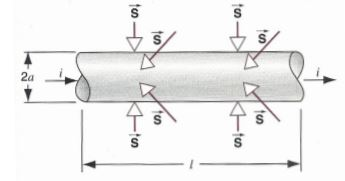
\includegraphics[scale=.8]{51m12pic.jpg}
\end{center}
\end{problem}

\vfill

\begin{solution}
\end{solution}

\end{document}